\documentclass[12pt]{article}

\usepackage[T1]{fontenc}
\usepackage[polish]{babel}
\usepackage[utf8]{inputenc}
\usepackage{lmodern} %zazwyczaj używam tej czcionki
%\usepackage{mathptmx} %times new roman
%\usepackage{helvet}
\usepackage{amsmath}	%pakiet z symbolami matematycznymi
\usepackage{graphicx}	%do wstawiania rysunków
\usepackage{float}	%do umiejscowienia rysunków w dobrych miejscach
\usepackage{wrapfig} %do wstawiania obrazków obok tekstu
\usepackage{caption}
\usepackage{subcaption}
%\usepackage{indentfirst}	%do zaczynania pierwszego akapitu wcięciem
\usepackage{multirow}	%do tabel
\usepackage{hyperref}	%refy działają jak hyperlinki
\usepackage{caption}	%przy refie idze na góre obrazka
\usepackage[table,xcdraw]{xcolor}
\selectlanguage{polish}	%język
\graphicspath{ {./obrazki/} }	%folder gdzie znajdują się rysunki
\hypersetup{
	colorlinks   = true, %Colours links instead of ugly boxes
	urlcolor     = blue, %Colour for external hyperlinks
	linkcolor    = blue, %Colour of internal links
	citecolor    = red %Colour of citations
}
\bibliographystyle{abbrv}
\renewcommand{\familydefault}{lmss}

\title{Komunikacja człowiek komputer - sprawozdania z aplikacji Mask Detector}
\author{Gorgoń Adam - 145278\\Grochowska Paulina - 145284}
\begin{document}
	\maketitle
	
	\section{Wstęp}
	\section{Prezentacja aplikacji}
	\section{Dane}
	\section{Użyte modele}
	Do wykrywania twarzy użyliśmy wytrenowanego modelu z biblioteki \href{https://opencv.org/}{OpenCV} w frameworku Caffe\cite{jia_caffe_2014}. Do klasyfikacji, czy osoba posiada maskę stworzyliśmy własną się konwolucyjną zbudowaną na technologi tensorflow\cite{tensorflow2015-whitepaper}. Model trenował się na cpu 3 godziny. Wczytywał zdjęcia z wcześniej wspomnianej bazy. Proporcje zbioru treningowego do testowego, wynosiły 0.8/0.2. Do lepszego wytrenowania model generował sobie zdjęcia, obracając zdjęcia o maksymalnie 15 stopni, robiąc lustrzane odbicie oraz przesuwając w pionie lub poziomie o 0.1 zdjęcia.
	\section{Działanie programu}
		\subsection{Przygotowanie zdjęcia do modelu}
		Wczytane zdjęcie jest zmieniane na tablicę jako RBG. Następnie układ jest zmieniany na BGR. Wynika to z faktu, że podczas trenowania dane były wczytywane za pomocą biblioteki \href{https://opencv.org/}{OpenCV}(wczytuje bgr), a w aplikacji przez \href{https://pillow.readthedocs.io/en/stable/}{Pillow}(wczytuje rgb).
		
		Następnie rozjaśniamy obraz za pomocą korekcji gamma, by zmniejszyć efekt cienia na zdjęciu.
		\begin{figure}
			\centering
			\begin{subfigure}[b]{0.49\textwidth}
				\centering
				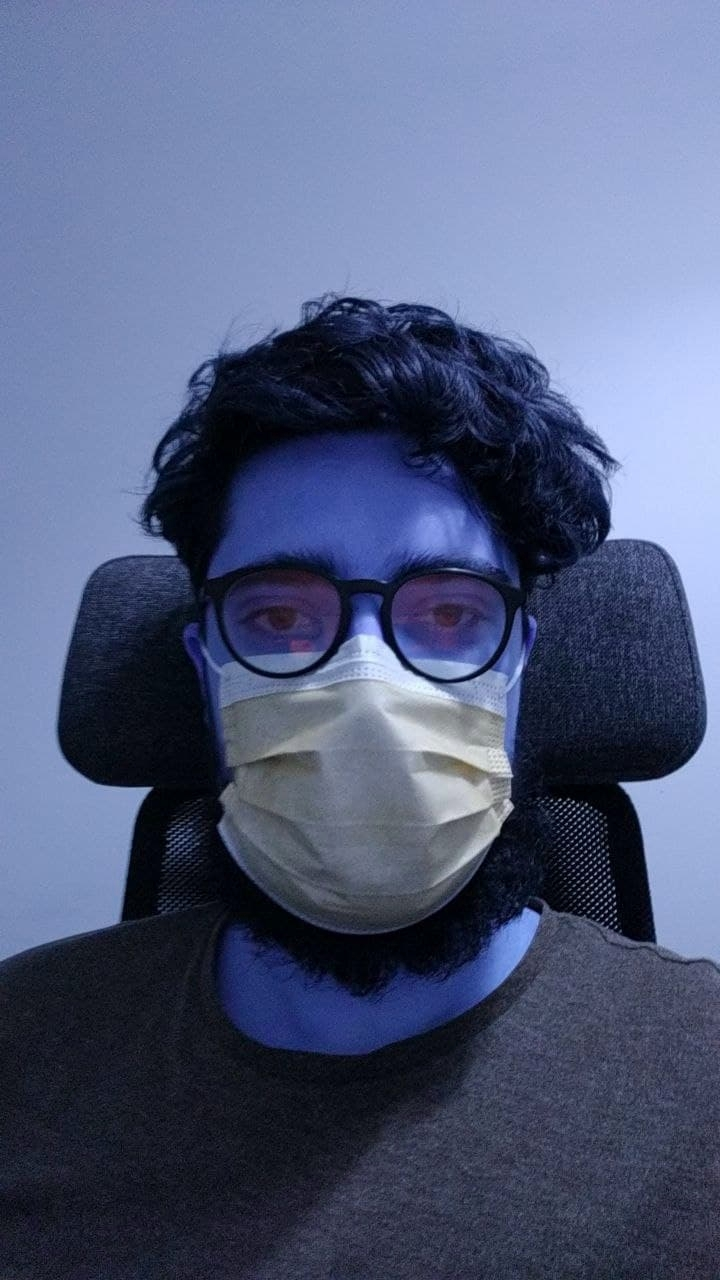
\includegraphics[width=0.45\textwidth]{rgb_to_bgr.jpeg}
				\caption{Zdjęcie bez obróbki z źle wczytanymi kolorami}
				\label{fig:bgr}
			\end{subfigure}
			\hfil
			\begin{subfigure}[b]{0.49\textwidth}
				\centering
				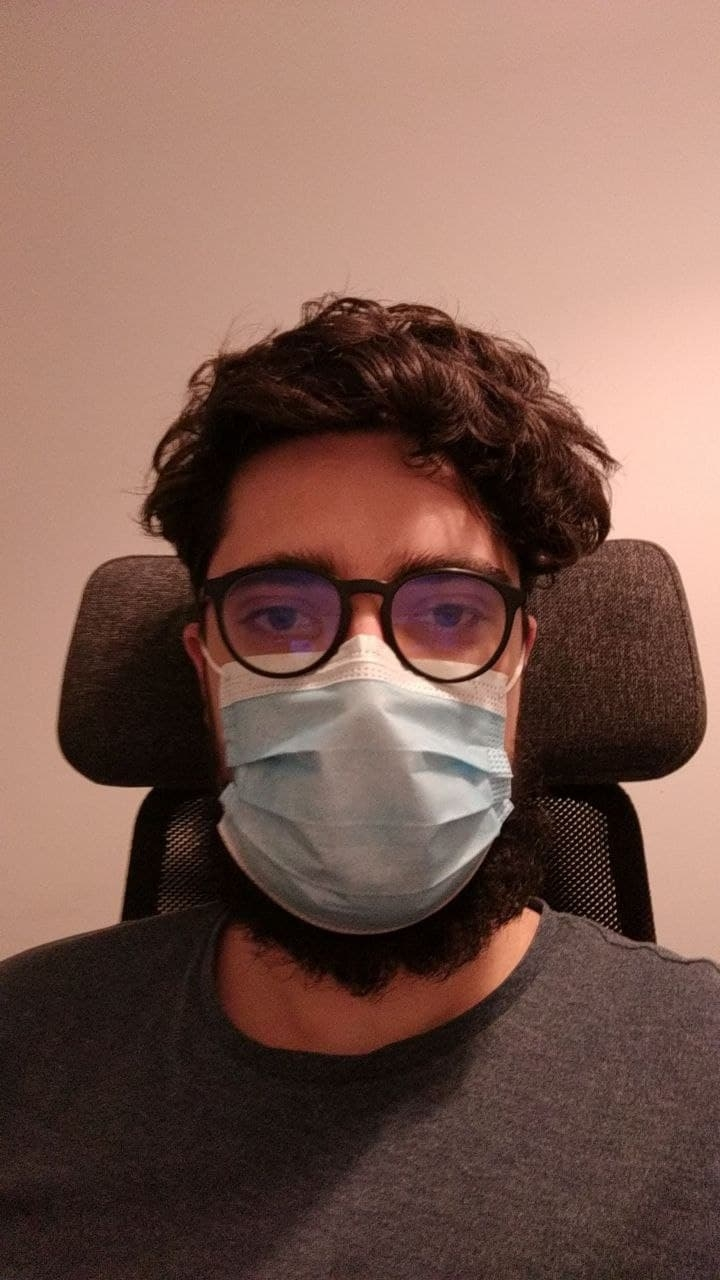
\includegraphics[width=0.45\textwidth]{nieprzerobione.jpeg}
				\caption{Zdjęcie bez obróbki z dobrze wczytanymi kolorami}
				\label{fig:nieprzerobione}
			\end{subfigure}
			\caption{Wczytywanie zdjęcia}
		\end{figure}
		\begin{figure}
			\centering
			\begin{subfigure}[b]{0.49\textwidth}
				\centering
				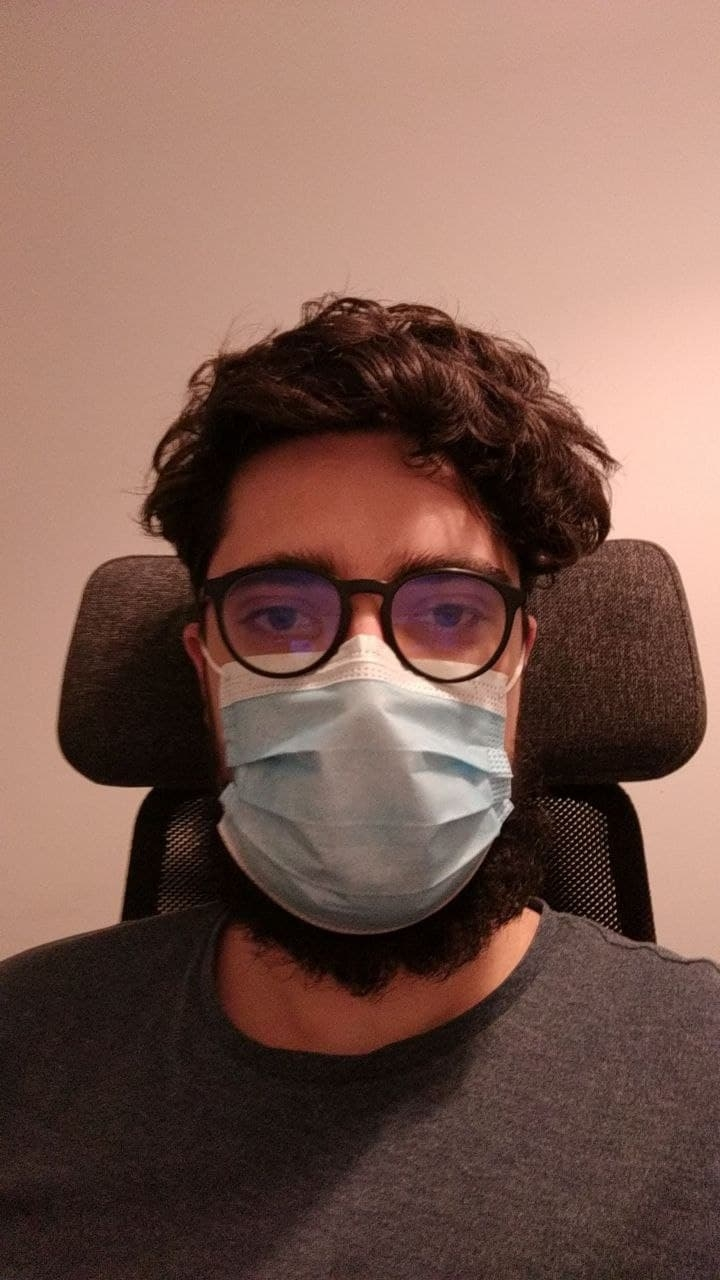
\includegraphics[width=0.45\textwidth]{nieprzerobione.jpeg}
				\caption{Przed}
				\label{fig:przed_gamma}
			\end{subfigure}
			\hfil
			\begin{subfigure}[b]{0.49\textwidth}
				\centering
				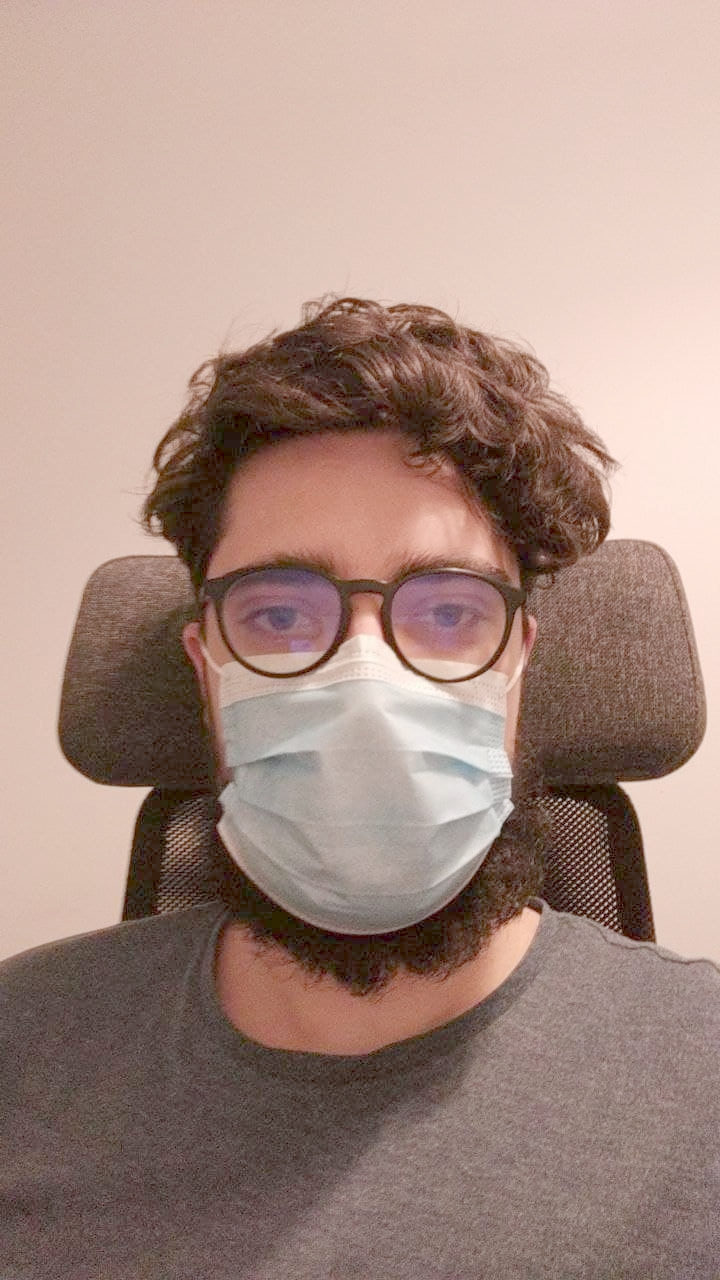
\includegraphics[width=0.45\textwidth]{po_gamma.jpeg}
				\caption{Po}
				\label{fig:po_gamma}
			\end{subfigure}
			\caption{Korekcja gamma}
		\end{figure}
		\subsection{Detekcja twarzy}
		Model sprawdza na zdjęciu czy znajduję się twarz. Jeśli pewność algorytmu na to, że w przeszukiwanym w tym momencie prostokącie znajduje się twarz, wynosi ponad 0.5, to program przechodzi do klasyfikacji.
		\subsection{Klasyfikacja twarzy}
		Jeśli program znajdzie twarz, to "wycina" prostokąt uznany za twarz, zmienia jego rozmiar na 124x124 i wysyła do sieci konwolucyjnej. Sieć wyrzuca liczbę w zakresie \([0, 1]\). Jeśli liczba jest mniejsza od 0.5, to twarz ma na sobie założoną maskę, w przeciwnym razie algorytm uznaje, że na twarzy nie ma maseczki.
		\begin{figure}
			\centering
			\begin{subfigure}[b]{0.49\textwidth}
				\centering
				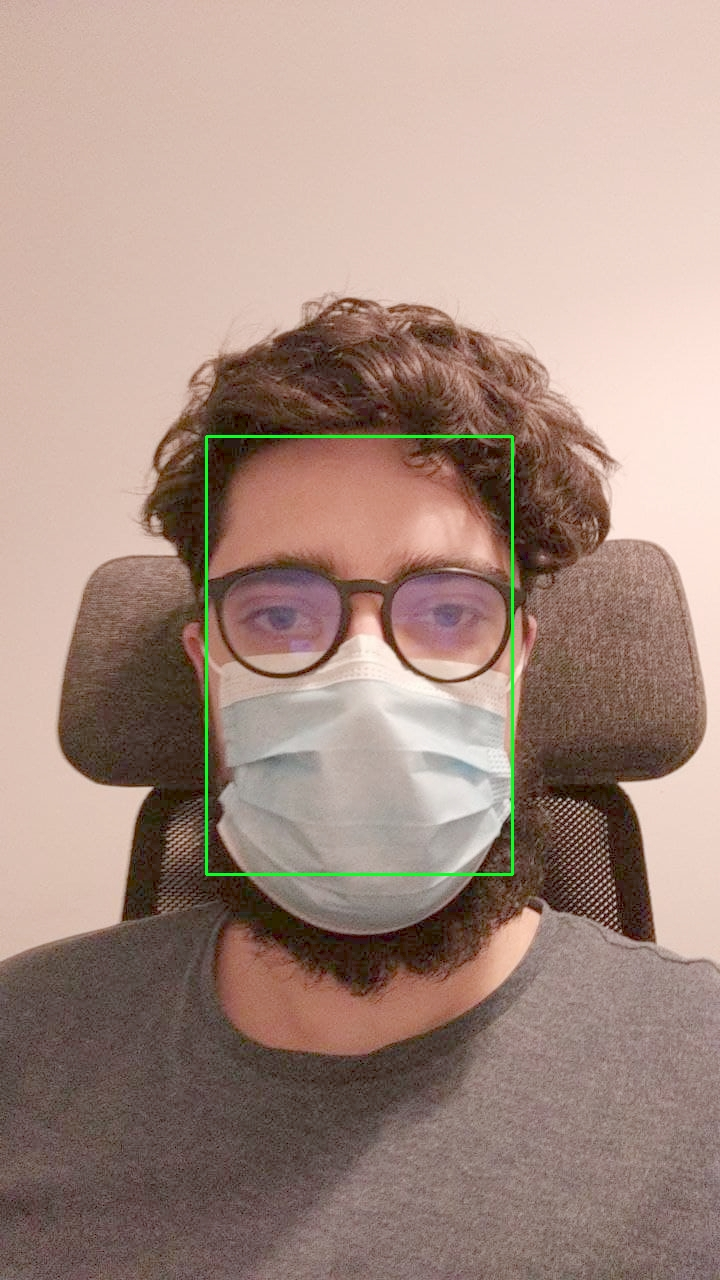
\includegraphics[width=0.45\textwidth]{twarz.jpeg}
				\caption{Algorytm znalazł twarz}
				\label{fig:twarz}
			\end{subfigure}
			\hfil
			\begin{subfigure}[b]{0.49\textwidth}
				\centering
				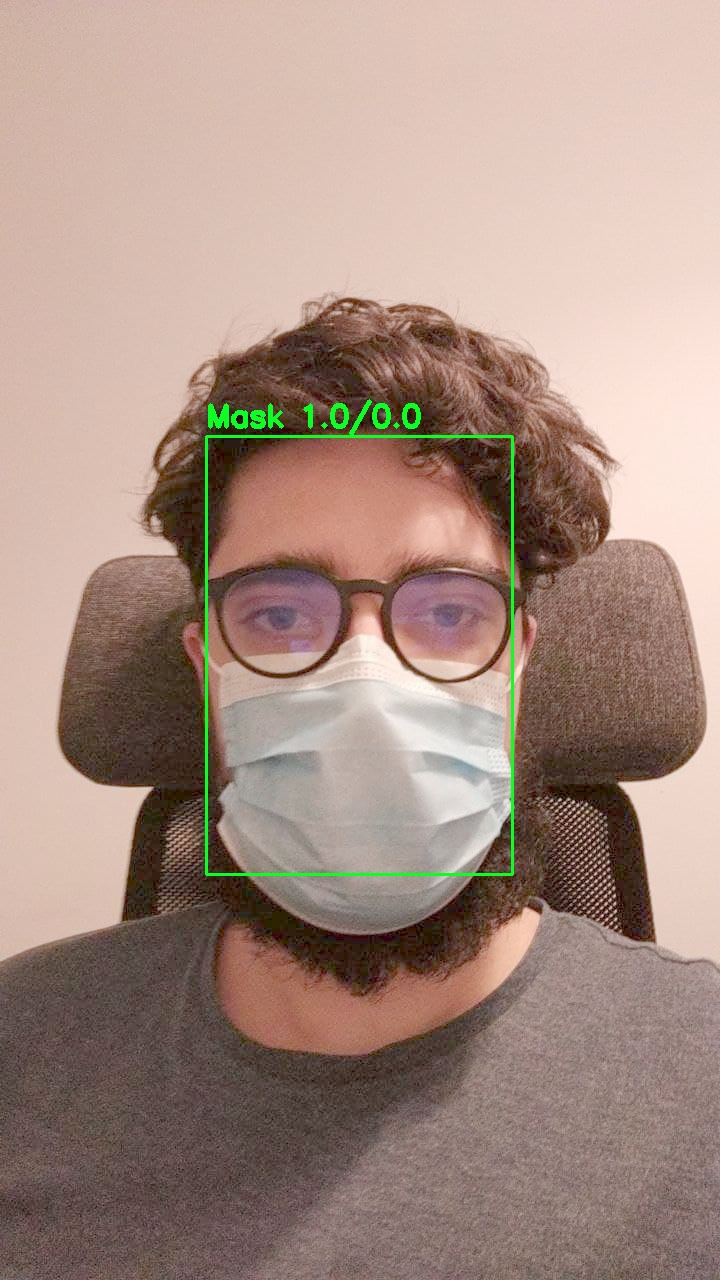
\includegraphics[width=0.45\textwidth]{maska.jpeg}
				\caption{Algorytm sklasyfikował twarz}
				\label{fig:maska}
			\end{subfigure}
			\caption{Działanie modelu}
		\end{figure}
	\section{Podsumowanie}
	\bibliography{md_bibl.bib}
\end{document}